\chapter[Cinematica delle velocità]{Cinematica delle velocità \\ \large \textit{Differential Kinematics}}

La cinematica delle velocità (o cinematica differenziale) di un manipolatore è rappresentata dall’insieme di \textbf{relazioni che legano le velocità dei giunti alla velocità della punta operativa}, ovvero le relazioni fra la velocità nello spazio dei giunti e la velocità nello spazio operazionale.\\
Anche in questo caso abbiamo la relazione di cinematica diretta ($\dot{\boldsymbol{q}} \rightarrow \dot{\boldsymbol{x}}_e$) e di cinematica inversa ($\dot{\boldsymbol{q}} \leftarrow \dot{\boldsymbol{x}}_e$).

Mentre non ci sono ambiguità nella definizione della velocità nello spazio dei giunti, rappresentata dal vettore $\boldsymbol{\dot{q}}$ , è necessario chiarire che cosa si intende per velocità nello spazio operazionale:
\begin{itemize}
	\item \textbf{Velocità in senso geometrico}: si considera in tal caso il vettore $\boldsymbol{v} = (\boldsymbol{\dot{p}}, \boldsymbol{\omega}) \in \R^6$ delle velocità geometriche, formato dalla velocità lineare $\bm{\dot{p}} \in \R^3$ e dalla velocità angolare $\bm{\omega} \in \R^3$ della punta operativa
	\item \textbf{Velocità in senso analitico}: si definisce in tal caso come velocità nello spazio operazionale il vettore $\bm{\dot{x}}\in\R^6$ ottenuto derivando rispetto al tempo il vettore $\boldsymbol{x} = \bm{k}(\bm{q}) = (\boldsymbol{p}, \boldsymbol{\phi}) \in \R^6$ delle coordinate operazionali (determinate dalla cinematica diretta delle posizioni)
\end{itemize}


Notiamo che in entrambi i casi la parte lineare è identica (esprime la velocità lineare della punta operativa lungo le direzioni degli assi del sistema di riferimento $\mathcal{R}_0$). \textbf{La parte relativa all'orientamento}, invece, \textbf{differisce} (in generale $\bm{\omega} \neq \bm{\dot{\phi}}$):
\begin{itemize}
	\item $\bm{\omega}$ corrisponde alla velocità angolare della punta
	(secondo le tre componenti relative agli assi di $\mathcal{R}_0$). È un "vero" vettore: $\bm{\omega}(t) = \bm{\omega}_1(t) + \dots + \bm{\omega}_n(t)$
	\item $\bm{\dot{\phi}}$ rappresenta la velocità con cui varia l’orientamento della punta, espressa come derivata rispetto al tempo dei tre angoli $(\phi, \theta, \psi)$ (Eulero o RPY) della rappresentazione minima dell’assetto. A differenza di $\bm{\omega}$ questo non è un "vero" vettore, visto che $\bm{\phi}(t) \neq \bm{\phi}_1(t) + \dots + \bm{\phi}_n(t)$ ma (al contrario del precedente, essendo questa una derivata) $\int \bm{\dot{\phi}}(\tau) d\tau = \bm{\phi}(\tau)$
\end{itemize}
\ \\


In entrambi i casi i due vettori delle sono \textbf{funzioni lineari} delle velocità ai giunti, quindi:
\begin{align}
	\bm{v} &= \bm{J}(\bm{q})\dot{\bm{q}} \label{eq:geom_jacob} \\ 
	\bm{\dot{x}} &= \bm{J}_A(\bm{q})\dot{\bm{q}} \label{eq:analy_jacob}
\end{align}
dove le due matrici sono rispettivamente chiamate \textbf{Jacobiano geometrico} e \textbf{Jacobiano analitico}. Inoltre, per entrambe, posto $n=\text{numero giunti}$:
$$
\bm{J},\bm{J}_A \in \R^{6\times n}
$$

\textbf{Quindi, risolvere il problema della cinematica diretta delle velocità significa determinare $\bm{J}$ o $\bm{J}_A$}. \\
Importante notare anche che entrambi gli Jacobiani dipendono dalla configurazione corrente del robot, visto che sono funzioni di $\bm{q}$.




\section{Jacobiano geometrico}
Iniziamo studiando un modo per ricavare lo Jacobiano geometrico. Da (\ref{eq:geom_jacob}) richiamiamo:
\begin{equation}\label{eq:geom_jacob_2}
\bm{v} 
=
\begin{bmatrix*}
\dot{\bm{p}} \\
\bm{\omega}
\end{bmatrix*}
=
\bm{J}(\bm{q})\dot{\bm{q}} 
=
\begin{bmatrix*}
	\bm{J}_p(\bm{q}) \\
	\bm{J}_o(\bm{q}) 
\end{bmatrix*}
\dot{\bm{q}}
\end{equation}
dove abbiamo indicato la scomposizione dello Jacobiano nelle 2 sottomatrici $3\times n$ relative alla sola posizione e orientamento.

\begin{figure}[H]
	\centering
	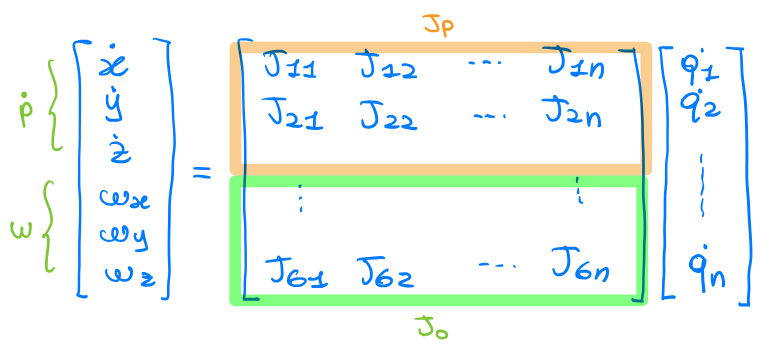
\includegraphics[width=0.6\linewidth]{images/diff_kine_1}
	\caption{Jacobiano geometrico}
	\label{fig:diffkine1}
\end{figure}
In primis possiamo iniziare osservando i contributi di ogni riga e ogni colonna:
\begin{itemize}
	\item \textbf{Righe}: ogni riga specifica l'effetto di \underline{tutti} i giunti sulla particolare velocità
	\item \textbf{Colonne}: ogni colonna, invece, identifica l'effetto del \underline{singolo} giunto su tutte le velocità
\end{itemize}

\vspace*{5pt}
\textit{\small Esempio:}\\
\textit{
\small
Se la colonna $i$ è completamente nulla, avremmo che il giunto $i$ \underline{non} avrà alcun effetto nella produzione di velocità dell'end-effector.\\
Invece se abbiamo una colonna nulla, e.g. la $1^a$, avremmo che il nostro robot \underline{non} produrrà alcuna velocità (e quindi nessun movimento) lungo $x$.
}

\vspace*{5pt}
Anche dall'esempio possiamo intuire la grande utilità dello Jacobiano: \textbf{tramite questa matrice possiamo facilmente identificare quali velocità dei giunti influenzeranno maggiormente velocità operazionali}, oltre ad esempio, a rendere più facile l'inversione cinematica ($v = J(q)\dot{q} \implies \dot{q} = J^{-1}(q)v \implies q = \int \dot{q} = \int J^{-1}(q)v$), che vedremo più avanti.



\subsection{Costruzione dello Jacobiano geometrico}
Per comprendere come “"costruire" lo Jacobiano geometrico, è utile determinare l’espressione della velocità (lineare ed angolare) di un singolo braccio.\\
Si consideri il generico braccio $i$, facente parte di una catena cinematica aperta, per la quale sono stati definiti i sistemi di riferimento secondo le convenzioni di DH.

\begin{figure}[H]
	\centering
	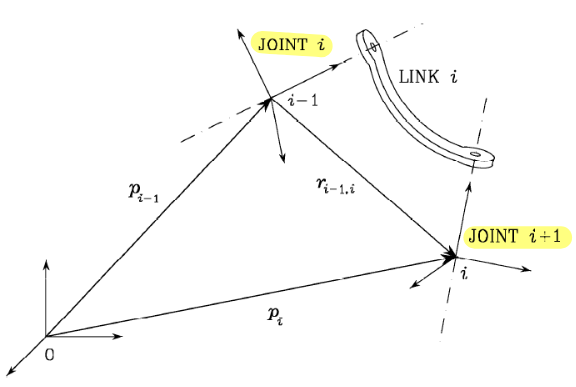
\includegraphics[width=0.5\linewidth]{images/diff_kine_2}
	\label{fig:diffkine2}
\end{figure}

Con riferimento alla figura sopra, possiamo affermare:
\begin{align*}
	\bm{\dot{p}}_i &= \bm{\dot{p}}_{i-1} + \bm{v}_{i-1, i} + \bm{\omega}_{i-1} \times \bm{r}_{i-1, i} \\
	\bm{\omega}_i &= \bm{\omega}_{i-1} + \bm{\omega}_{i-1, i}
\end{align*}
dove $\bm{v}_{i-1, i} \triangleq \bm{\dot{r}}_{i-1, i}$ (per dim. vedi slide in italiano).\\


Nel caso di un \textbf{giunto prismatico} abbiamo:
\begin{align*}
	\begin{cases}
		\bm{\omega}_{i-1,i} = 0 \\ 
		\bm{v}_{i-1, i} = \dot{\bm{d}}_i\bm{z}_{i-1}
	\end{cases}
	\implies
	\begin{cases}
		\bm{\dot{p}}_i = \bm{\dot{p}}_{i-1} + \dot{\bm{d}}_i\bm{z}_{i-1} + \bm{\omega}_{i-1} \times \bm{r}_{i-1, i} \\
		\bm{\omega}_i = \bm{\omega}_{i-1}
	\end{cases}
\end{align*}

mentre per un \textbf{giunto rotoidale}:
\begin{align*}
	\begin{cases}
		\bm{\omega}_{i-1,i} = \dot{\bm{\theta}}_i\bm{z}_{i-1} \\ 
		\bm{v}_{i-1, i} = \bm{\omega}_{i-1,i} \times \bm{r}_{i-1, i}
	\end{cases}
	\implies
	\begin{cases}
		\bm{\dot{p}}_i = \bm{\dot{p}}_{i-1} + \bm{\omega}_{i} \times \bm{r}_{i-1, i} \\
		\bm{\omega}_i = \bm{\omega}_{i-1} + \dot{\bm{\theta}}_i\bm{z}_{i-1}
	\end{cases}
\end{align*}

%Di conseguenza, richiamando (\ref{eq:geom_jacob_2}): $\begin{bmatrix*}\dot{\bm{p}} \\	\bm{\omega}\end{bmatrix*}=\bm{J}(\bm{q})\dot{\bm{q}}$ possiamo osservare che abbiamo trovato le due componenti di

Richiamando la fig. \ref{fig:diffkine1} e (\ref{eq:geom_jacob_2}), possiamo scomporre la matrice $\bm{J}$ come segue:
$$
\bm{J}(\bm{q})\dot{\bm{q}}
=
\begin{bmatrix*}
	\bm{J}_p(\bm{q}) \\
	\bm{J}_o(\bm{q}) 
\end{bmatrix*}
\dot{\bm{q}}
=
\begin{bmatrix*}
	\bm{J}_{p,1} & \bm{J}_{p,2} & \cdots & \bm{J}_{p,n} \\
	\bm{J}_{o,1} & \bm{J}_{o,1} & \cdots & \bm{J}_{o,n}
\end{bmatrix*}
\begin{bmatrix*}
	\dot{q}_1 \\ \dot{q}_2 \\ \vdots \\ \dot{q}_n
\end{bmatrix*}
$$
dove $\bm{J}_{p,i}$, $\bm{J}_{o,i} \in \R^3$ sono le colonne di $\bm{J}_p$ e $\bm{J}_o$ (per semplicità di notazione abbiamo omesso la dipendenza da $q$). Da qui poi possiamo scrivere:
$$
\bm{\dot{p}} = \sum_{i=1}^n \bm{J}_{p,i} \dot{q}_i
\qquad , \qquad
\bm{\omega} = \sum_{i=1}^n \bm{\omega}_{i-1, i} = \sum_{i=1}^n \bm{J}_{o,i} \dot{q}_i
$$
e quindi:

\begin{itemize}
	\item Nel caso di un \textbf{giunto prismatico} ($q_i = d_i$):
	\begin{align*}
		\begin{cases}
			\bm{J}_{p,i}\dot{q}_i = \bm{v}_{i-1,i} = \dot{d}_i \bm{z}_{i-1} \\
			\bm{\omega}_{i-1, i} = 0
		\end{cases}
		\implies
		\begin{cases}
			\bm{J}_{p,i} = \bm{z}_{i-1} \\
			\bm{J}_{o,i} = \bm{0}
		\end{cases}
	\end{align*}
	\item Mentre per un \textbf{giunto rotoidale} ($q_i = \theta_i$):
	\begin{align*}
		\begin{cases}
			\bm{J}_{p,i}\dot{q}_i = \bm{v}_{i-1,i} = \bm{\omega}_{i-1,i} \times \bm{r}_{i-1,e} = \dot{\bm{\theta}}_i\bm{z}_{i-1} \times (\bm{p}_e - \bm{p}_{i-1}) \\
			\bm{\omega}_{i-1,i} = \dot{\bm{\theta}}_i\bm{z}_{i-1}
		\end{cases}
		\implies
		\begin{cases}
			\bm{J}_{p,i} = \bm{z}_{i-1} \times (\bm{p}_e - \bm{p}_{i-1}) \\
			\bm{J}_{o,i} = \bm{z}_{i-1}
		\end{cases}
	\end{align*}
\end{itemize}


\vspace*{10pt}
Riassumendo:

\setlength{\fboxsep}{0pt} % Adjust the padding as needed
\fbox{
	\begin{minipage}{\textwidth}
		\begin{align*}
			\text{i-th column of } \bm{J}
			=
			\begin{bmatrix}
				\bm{J}_{p,i} \\
				\bm{J}_{o,i}
			\end{bmatrix}
			=
			\begin{cases}
				\begin{bmatrix}
					\bm{z}_{i-1} \\
					\bm{0}
				\end{bmatrix}
				& \textit{for a \textbf{prismatic} joint}
				\vspace*{5pt}
				\\
				\begin{bmatrix}
					\bm{z}_{i-1} \times (\bm{p} - \bm{p}_{i-1}) \\
					\bm{z}_{i-1} 
				\end{bmatrix}
				& \textit{for a \textbf{revolute} joint}
			\end{cases}
		\end{align*}
		\vspace*{2pt}
	\end{minipage}
}



\vspace*{25pt}
\subsubsection{Costruzione pratica}
Nella pratica, per trovare i vettori della formula di cui sopra, possiamo fare delle osservazioni.

\begin{itemize}
	\item $\bm{z}_{i-1} = 3^{a} \text{ colonna di } {}^0\bm{R}_{i-1} = {}^0\bm{R}_{1} \cdots {}^{i-2}\bm{R}_{i-1}$.
	\item $\bm{p}_e = \text{primi 3 elementi dell'ultima colonna di } {}^0\bm{T}_n = {}^0\bm{T}_{1} \cdots {}^{n-1}\bm{T}_{}$
	\item $\bm{p}_{i-1} = \text{primi 3 elementi dell'ultima colonna di } {}^0\bm{T}_{i-1} = {}^0\bm{T}_{1} \cdots {}^{i-2}\bm{T}_{i-1}$
\end{itemize}

\vspace*{10pt}
\textit{Esempio}\\
\textit{Per semplicità non useremo il grassetto per i vettori e} $p \equiv p_e$. \textit{Come si vede dalla figura abbiamo tutti giunti rotoidali.}
\begin{figure}[H]
	\centering
	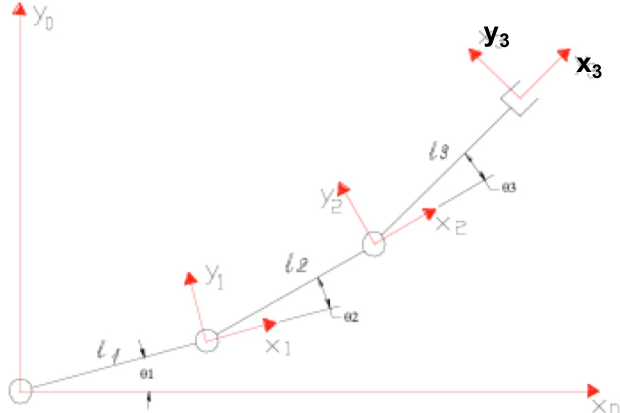
\includegraphics[width=0.4\linewidth]{images/diff_kine_3}
	\label{fig:diffkine3}
\end{figure}
$$
J(q)
=
\begin{bmatrix*}
z_0 \times (p - p_0) & z_1 \times (p - p_1) & z_2 \times (p - p_2) \\
z_0 & z_1 & z_2
\end{bmatrix*}
$$
\textit{e quindi}:
\begin{equation*}  
	{}^0T_0
	=
	\begin{bmatrix}
		1 & 0 & \cellcolor{cyan}0 & \cellcolor{yellow}0 \\
		0 & 1 & \cellcolor{cyan}0 & \cellcolor{yellow}0 \\
		0 & 0 & \cellcolor{cyan}1 & \cellcolor{yellow}0 \\
		0 & 0 & 0 & 1 \\
	\end{bmatrix}
	\implies
	\colorbox{cyan}{$z_0$}
	=
	\begin{bmatrix}
		0 \\ 0 \\ 1
	\end{bmatrix}
	\ , \
	\colorbox{yellow}{$p_0$}
	=
	\begin{bmatrix}
		0 \\ 0 \\ 0
	\end{bmatrix}
\end{equation*}

\begin{equation*}
	{}^0T_1
	=
	\begin{bmatrix}
		c_1 & -s_1 & \cellcolor{cyan}0 & \cellcolor{yellow}l_1 c_1 \\
		s_1 & c_1 & \cellcolor{cyan}0 & \cellcolor{yellow}l_1 s_1 \\
		0 & 0 & \cellcolor{cyan}1 & \cellcolor{yellow}0 \\
		0 & 0 & 0 & 1 \\
	\end{bmatrix}
	\implies
	\colorbox{cyan}{$z_1$}
	=
	\begin{bmatrix}
		0 \\ 0 \\ 1
	\end{bmatrix}
	\ , \
	\colorbox{yellow}{$p_1$}
	=
	\begin{bmatrix}
		l_1 c_1 \\ l_1 s_1 \\ 0
	\end{bmatrix}
\end{equation*}

\begin{equation*}
	{}^0T_2
	=
	\begin{bmatrix}
		c_{12} & -s_{12} & \cellcolor{cyan}0 & \cellcolor{yellow}l_1 c_1 + l_2c_{12}\\
		s_{12} & c_{12} & \cellcolor{cyan}0 & \cellcolor{yellow}l_1 s_1 + l_2s_{12}\\
		0 & 0 & \cellcolor{cyan}1 & \cellcolor{yellow}0 \\
		0 & 0 & 0 & 1 \\
	\end{bmatrix}
	\implies
	\colorbox{cyan}{$z_2$}
	=
	\begin{bmatrix}
		0 \\ 0 \\ 1
	\end{bmatrix}
	\ , \
	\colorbox{yellow}{$p_2$}
	=
	\begin{bmatrix}
		l_1 c_1 + l_2c_{12} \\ l_1 s_1 + l_2s_{12} \\ 0
	\end{bmatrix}
\end{equation*}

\begin{equation*}
	{}^0T_3
	=
	\begin{bmatrix}
		c_{123} & -s_{123} & 0 & \cellcolor{yellow}l_1 c_1 + l_2c_{12} + l_3c_{123}\\
		s_{123} & c_{123} & 0 & \cellcolor{yellow}l_1 s_1 + l_2s_{12} + l_3s_{123}\\
		0 & 0 & 1 & \cellcolor{yellow}0 \\
		0 & 0 & 0 & 1 \\
	\end{bmatrix}
	\implies
	\colorbox{yellow}{$p$}
	=
	\begin{bmatrix}
		l_1 c_1 + l_2c_{12} + l_3c_{123} \\ l_1 s_1 + l_2s_{12} + l_3s_{123} \\ 0
	\end{bmatrix}
\end{equation*}

\vspace*{10pt}
\textit{Ora dobbiamo solo calcolarci le differenze ed i prodotti vettoriali per trovare} $J(q)$:
\begin{figure}[H]
	\centering
	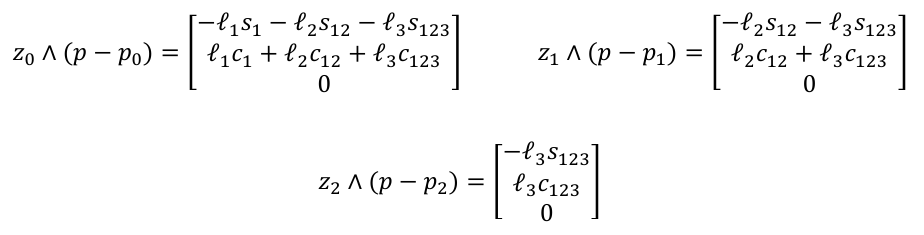
\includegraphics[width=0.8\linewidth]{images/diff_kine_4}
	\label{fig:diffkine4}
\end{figure}
\vspace*{-30pt}
$$
\Downarrow
$$
\begin{figure}[H]
	\centering
	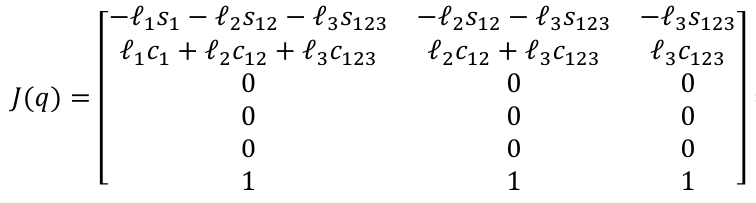
\includegraphics[width=0.6\linewidth]{images/diff_kine_5}
	\label{fig:diffkine5}
\end{figure}

\textit{In questo esempio possiamo già vedere l'esempio di un robot \textbf{sottoattuato}: a causa di tutti quegli 0 nella Jacobiana non possiamo controllare in alcun modo $\dot{z}, \omega_y, \omega_z$. In realtà in questo caso il risultato era atteso visto che abbiamo analizzato un manipolatore planare (2D) in 3D.\\ In questo caso è possibile utilizzare una rappresentazione ridotta di $J(q)$, levando le righe nulle (ovviamente bisogna ricordarci che è la versione ridotta)}.




\section{Jacobiano analitico}
Lo Jacobiano analitico viene calcolato dall’applicazione della sua stessa definizione, derivando rispetto al tempo il vettore $\bm{p}(\bm{q})$ ottenuto dalla cinematica diretta delle posizioni:	
\begin{gather*}
	\dot{\bm{x}}
	=
	\frac{d\bm{x}}{dt}
	=
	\underbrace{\frac{\partial\bm{x}}{\partial \bm{q}}}_{\bm{J}_A(\bm{q})}
	\underbrace{\frac{d\bm{q}}{d t}}_{\dot{\bm{q}}}
	=
	\bm{J}_A(\bm{q})\dot{\bm{q}}
\end{gather*}
E ${\partial\bm{x}} / {\partial \bm{q}}$ (che è proprio lo Jacobiano analitico) non è altro che lo Jacobiano (nel senso inteso ad analisi):
\[
\bm{J} = \frac{\partial \bm{f}}{\partial \bm{x}} =
\begin{bmatrix}
	\frac{\partial f_1}{\partial x_1} & \frac{\partial f_1}{\partial x_2} & \cdots & \frac{\partial f_1}{\partial x_n} \\[7pt]
	\frac{\partial f_2}{\partial x_1} & \frac{\partial f_2}{\partial x_2} & \cdots & \frac{\partial f_2}{\partial x_n} \\[5pt]
	\vdots & \vdots & \ddots & \vdots \\[5pt]
	\frac{\partial f_m}{\partial x_1} & \frac{\partial f_m}{\partial x_2} & \cdots & \frac{\partial f_m}{\partial x_n}
\end{bmatrix}
\]

\vspace*{10pt}
\subsubsection{Conversione $\bm{J}(\bm{q}) \leftrightarrow \bm{J}_A(\bm{q})$}
Data la rappresentazione minima prescelta per l’assetto (Eulero, RPY) è possibile esprimere $\bm{\omega}$ in funzione di $\dot{\bm{\phi}}$ come:
$$
\bm{\omega} = \bm{T}(\bm{\phi})\bm{\dot{\phi}}
$$
e quindi $\bm{J}(\bm{q})$ in funzione di $\bm{J}_A(\bm{q})$:
$$
\bm{J}(\bm{q})
=
\begin{bmatrix*}
\bm{I} & \bm{0} \\
\bm{0} & \bm{T}(\bm{\phi})
\end{bmatrix*}
=
\bm{J}_A(\bm{q})
$$
(la forma di $\bm{T}(\bm{\phi})$ dipende dalla rappresentazione scelta per l'assetto).

I valori di $\bm{\phi}$ per cui il determinante della matrice $\bm{T}(\bm{\phi})$ si annulla nei vari casi corrispondono a singolarità della rappresentazione dell’assetto usata (\textbf{gimbal lock}). Questo significa che ci sono velocità angolari che non possono essere espresse per mezzo di $\dot{\bm{\phi}}$.


\vspace*{5pt}
\textit{Esempio \\ Se prendiamo gli angoli di Eulero ZYZ}:
\begin{figure}[H]
	\centering
	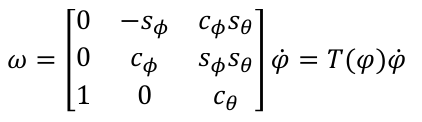
\includegraphics[width=0.4\linewidth]{images/diff_kine_6}
	\label{fig:diffkine6}
\end{figure}






\section{Singolarità cinematiche}
\textbf{Le configurazioni del manipolatore per cui lo Jacobiano (geometrico) non è di rango pieno sono dette singolarità cinematiche o configurazioni singolari}. Ovvero:
$$
\setlength{\fboxsep}{15pt}
\boxed{
\det(\bm{J}(\bm{q}_s)) = 0
\implies 
\bm{q}_s \text{ è una configurazione singolare}
}
$$

Le singolarità corrispondono a configurazioni in cui la mobilità del manipolatore è ridotta: 
\begin{itemize}
	\item Esistono velocità cartesiane che non possono essere ottenute da velocità ai giunti
	\item Velocità non nulle ai giunti generano velocità cartesiane nulle
\end{itemize}
Inoltre:
\begin{itemize}
	\item Quando il manipolatore è in configurazione singolare, il problema cinematico inverso può presentare infinite soluzioni
	\item In un intorno della singolarità, a piccole velocità della punta possono corrispondere grandi velocità dei giunti (poichè $v=J\dot{q} \implies \dot{q} = J^{-1}v \implies J^{-1} = \frac{1}{\det(J)} \text{adj}(J)$ e quindi se $\det(J) \to 0$ abbiamo $J^{-1} \to \infty$)
\end{itemize}

Le singolarità cinematiche possono essere:
\begin{itemize}
	\item \textbf{"di confine"}: i bracci del manipolatore sono completamente
	stesi o retratti, in una configurazione limite (“di confine”)
	dello spazio di lavoro
	\item \textbf{interne}: si trovano all’interno dello spazio di lavoro e
	corrispondono tipicamente all’allineamento di due o più assi
	di movimento dei giunti oppure a particolari configurazioni
\end{itemize}
Le configurazioni singolari interne sono le più critiche dal punto di vista pratico perché possono essere raggiunte ovunque all’interno dello spazio di lavoro durante l’esecuzione di una traiettoria pianificata nello spazio operazionale.


\subsection{Manipolatori con polso sferico}
Per i manipolatori con polso sferico le singolarità possono essere disaccoppiate in spalla e polso:
\begin{itemize}
	\item Per il \textbf{polso}, abbiamo singolarità quando 2 dei 3 assi si allineano, in particolare (con riferimento alla figura) $z_3$ e $z_5$. In generale, qualsiasi allineamento di due o più giunti rotanti porta ad una singolarità, poiché due rotazioni opposte di uguale entità non producono movimento nell'end-effector
	\begin{figure}[H]
		\centering
		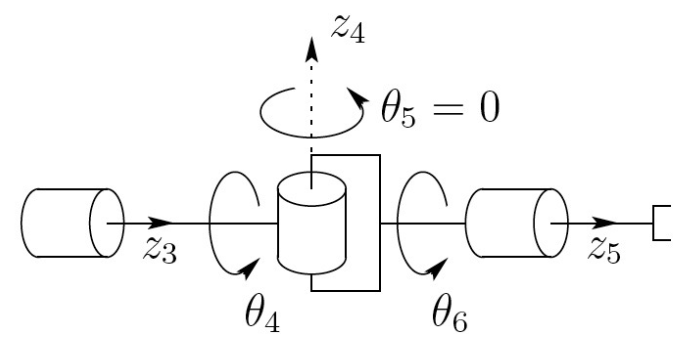
\includegraphics[width=0.35\linewidth]{images/diff_kine_7}
		\caption{Singolarità per $\theta_5 = 0, \pi$}
		\label{fig:diffkine7}
	\end{figure}
	\item Per la \textbf{spalla}, invece, possiamo analizzare le singolarità guardando il determinante di $\bm{J}_p$, che risulta nullo per $\theta_3=0,\pi$ (singolarità "di confine"):
	\begin{figure}[H]
		\centering
		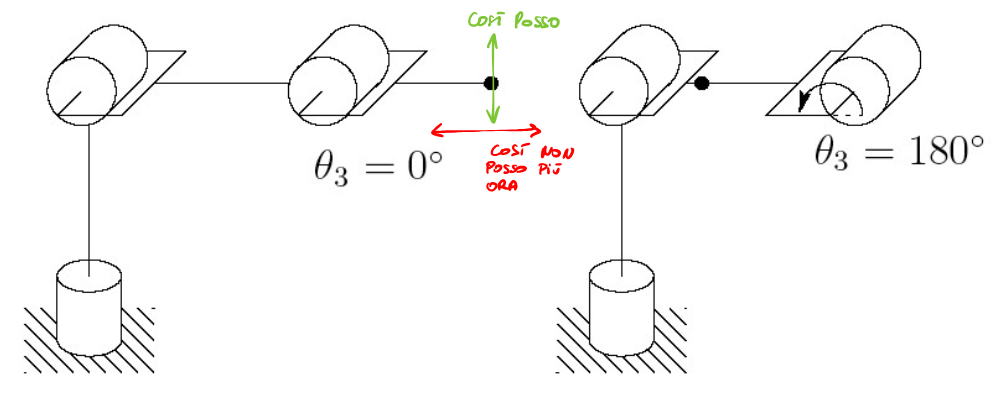
\includegraphics[width=0.4\linewidth]{images/diff_kine_8}
		\caption{Singolarità per $\theta_3=0,\pi$}
		\label{fig:diffkine8}
	\end{figure}
	oppure per $a_2c_2 + a_3c_{23}=0$ (singolarità interna):
	\begin{figure}[H]
		\centering
		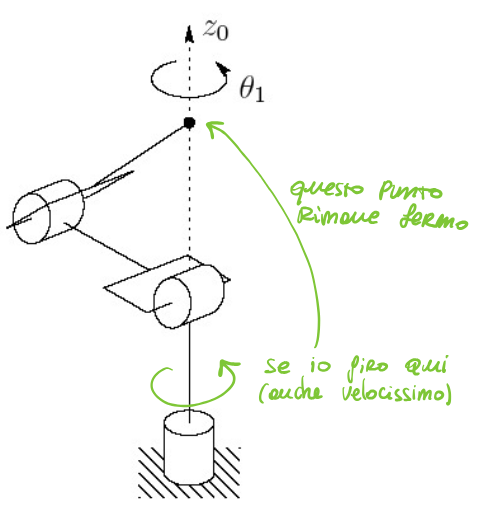
\includegraphics[width=0.35\linewidth]{images/diff_kine_9}
		\caption{Singolarità per $a_2c_2 + a_3c_{23}=0$}
		\label{fig:diffkine9}
	\end{figure}
	
\end{itemize}





\section{Ridondanza cinematica}

Un manipolatore è ridondante dal punto di vista cinematico se possiede un \textbf{numero di gradi di libertà maggiore del numero di variabili necessarie} per descrivere il compito che deve svolgere.

Un manipolatore è \textbf{intrinsecamente ridondante} se la dimensione $m$ del suo spazio operazionale è inferiore alla dimensione $n$ del suo spazio dei giunti. In generale, però, la ridondanza è un concetto relativo al compito assegnato al manipolatore (\textit{e.g. anche nel caso $m=n$ un manipolatore può risultare ridondante, come nel caso se per operare gli bastasse solo $x$ e $y$}).

Visto che $v = J(q)\dot{q}$ è un sistema lineare ($y = Ax$), possiamo analizzarlo utilizzando gli strumenti noti dell'algebra. Ricordiamo i seguenti concetti:
\begin{itemize}
	\item $\text{Im}(A) \equiv \text{span}(A) \equiv \mathcal{R}(A)$
	\item $\text{Ker}(A) \equiv \mathcal{N}(A) \triangleq \{ x : Ax = 0 \}$
	\item $A$ \textit{square} and $\det(A)\neq0 \iff \text{Ker}(A)=\{0\}$
	\item $A$ \textit{rectangular} $\implies \text{Ker}(A)\neq{\{0\}}$
\end{itemize}

Se un manipolatore è ridondante ($m > n$) abbiamo una matrice $J$ rettangolare:
$$
\bm{J}(\bm{q})
=
\begin{bmatrix}
	& & & & & & & & & \\
	& & & & & & & & & \\
\end{bmatrix}
=
\textit{rettangolare}
\implies
\text{Ker}(A)\neq{\{0\}}
$$
quindi, visto che il kernel \underline{non} è banale, da definizione avremo:
$$
\exists \bm{q} : \bm{J}(\bm{q}) = 0
$$ 
ovvero \textbf{esistono velocità dei giunti non nulle che non generano velocità nell'end-effector}.


\setlength{\fboxsep}{10pt} % Adjust the padding as needed
\fbox{
	\begin{minipage}{\textwidth}
		Da questa osservazione possiamo dire che:
		\vspace*{5pt}
		\begin{itemize}
			\item Il \textbf{range space} $\mathcal{R}(\bm{J}(\bm{q})) \in \R^m$ è quel sottospazio delle velocità dell'end-effector che possono essere generate da velocità ai giunti (per la postura corrente $\bm{q}$).
			\item Il \textbf{null space} $\mathcal{N}(\bm{J}(\bm{q})) \in \R^n$ è quel sottospazio delle velocità ai giunti che non producono alcuna velocità nell'end effector (per la postura corrente $\bm{q}$).
		\end{itemize}
	\end{minipage}
}


\vspace*{5pt}
\subsubsection{Altre cose dette da Rizzo}

Supponiamo $\dot{\bm{q}}^* \in \mathcal{N}(\bm{J}(\bm{q})) \implies \bm{J}(\bm{q})\dot{\bm{q}}^* = 0$. Allora, se poniamo $\bm{v} = \bm{J}(\bm{q})\dot{\bm{q}}$ abbiamo:
$$
\bm{v} = \bm{J}(\bm{q})(\dot{\bm{q}} + \dot{\bm{q}}^*) = \bm{J}(\bm{q})\dot{\bm{q}} + \cancelto{0}{\bm{J}(\bm{q})\dot{\bm{q^*}}} = \bm{J}(\bm{q})\dot{\bm{q}}
$$
Ora poniamo $\langle\dot{q}_1, \dot{q}_2, \dot{q}_3\rangle$ base di $\mathcal{N}(\bm{J}(\bm{q}))$. Grazie a questa terna, richiamando che ovviamente ora qualsiasi vettore ($\in \mathcal{N}(\bm{J}(\bm{q}))$) può essere scritto come $\alpha\dot{q}_1 + \beta\dot{q}_2 + \gamma\dot{q}_3$, possiamo definire:
$$
P \triangleq [ \dot{q}_1, \dot{q}_2, \dot{q}_3 ]
=
\text{matrice generatrice del null space}
$$
e quindi, qualsiasi $\dot{\bm{q}}^* \in \mathcal{N}(\bm{J}(\bm{q}))$ può essere scritto come:
$$
\dot{\bm{q}}^* = P\dot{q}_a \quad , \quad \dot{q}_a \text{ arbitrario}
$$






\section{Cinematica inversa delle velocità}
Il problema della cinematica inversa delle velocità consiste nel calcolo di $\dot{\bm{q}}$ partire dalla conoscenza di $\bm{v}$.

Se lo Jacobiano $\bm{J}(\bm{q})$ è \textbf{quadrato} e \textbf{full-rank}, il problema viene risolto semplicemente dall’equazione:
\begin{equation}\label{eq:diff_inv_kine}
\dot{\bm{q}} = \bm{J}^{-1}(\bm{q})\bm{v}
\end{equation}

Se, invece, siamo nel caso \textbf{rettangolare} e \textbf{non full-rank} (come nel caso di un manipolatore \textbf{ridondante}), dobbiamo trovare altri modi, ad esempio tramite la \textbf{right pseudo-inverse}:
\begin{align}\label{eq:diff_inv_kine_pseudo}
\dot{\bm{q}} = \bm{J}^{\dagger}(\bm{q})\bm{v}
\qquad
\textit{dove}
\qquad
\bm{J}^{\dagger} \triangleq \bm{J}^{T}(\bm{J} \bm{J}^{T})^{-1}
\end{align}


\subsection{Metodologie avanzate per il caso rettangolare/ridondante}
Soluzioni diverse possono essere ottenute ottimizzando la ricerca di $\dot{\bm{q}}$ con l’introduzione di opportuni funzionali di costo e di vincoli secondari, tali da permettere di sfruttare la ridondanza del manipolatore nell’esecuzione del compito.

Ad esempio:
\begin{align*}
\text{minimize} & \quad g(\dot{\bm{q}}) = \frac{1}{2} \dot{\bm{q}}^T \bm{W} \dot{\bm{q}} \\
\text{subject to} & \quad \bm{v} = \bm{J}(\bm{q})\bm{\dot{q}}
\end{align*}
dove $\bm{W}\in\R^{n\times n}$ è una matrice di pesi, simmetrica e definita positiva.\\
Tramite il metodo dei moltiplicatori di Lagrange (che ci permettono di includere il "subject to" dentro la funzione da minimizzare) possiamo ottenere una soluzione in forma chiusa per il problema dato:
$$
g(\dot{\bm{q}}, \lambda) = \frac{1}{2} \dot{\bm{q}}^T \bm{W} \dot{\bm{q}}
+ \lambda^T(\bm{v} - \bm{J}(\bm{q})\dot{\bm{q}})
$$
\begin{figure}[H]
	\centering
	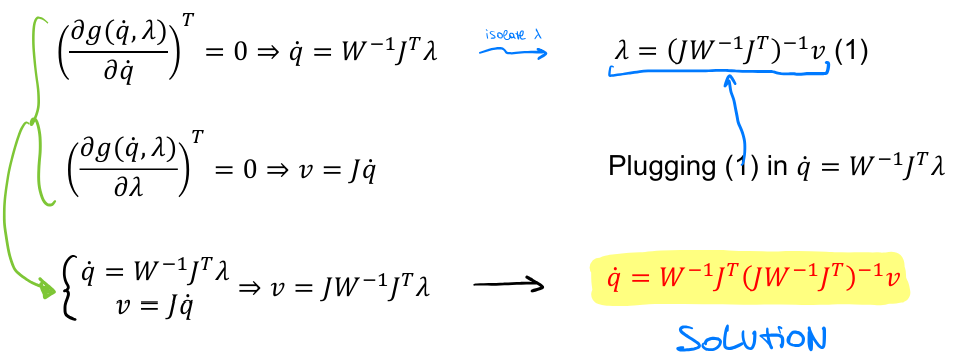
\includegraphics[width=0.7\linewidth]{images/diff_kine_10}
	\label{fig:diffkine10}
\end{figure}

Dove possiamo notare che ponendo $\bm{W} = \bm{I}$ questa soluzione è equivalente a quella con la pseudo-inversa destra.

Visto che lo Jacobiano rettangolare è relativo anche al caso di \textbf{manipolatori ridondanti}, nella nostra soluzione dovremmo tenere in considerazione le velocità non nulle dei giunti che non producono velocità dell'end-effector: riprendendo la soluzione (\ref{eq:diff_inv_kine_pseudo}), possiamo aggiungervi un qualsiasi vettore del null-space e rimarrà comunque valida:
\begin{equation*}
\dot{\bm{q}} = \bm{J}^{\dagger}(\bm{q})\bm{v}
+
\dot{\bm{q}}_n
\qquad
\textit{dove}
\qquad
\dot{\bm{q}}_n \in \mathcal{N}(\bm{J}(\bm{q}))
\tag{$\star$}
\end{equation*}
visto che l'ultimo termine è t.c. $\bm{J}(\bm{q})\dot{\bm{q}}_n = 0$:
$$
\bm{J}(\bm{q})
= 
\bm{J}(\bm{q})(\bm{J}(\bm{q})^{\dagger} \bm{v} + \bm{\dot{q}}_n)
=
\cancelto{I}{(\bm{J}(\bm{q}) (\bm{J}(\bm{q})^\dagger)} \bm{v} + \cancelto{0}{\bm{J}(\bm{q})\bm{\dot{q}}_n} = \bm{v}
$$

come scegliamo il vettore $\bm{\dot{q}}_n$? Possiamo usare un "trucco" accennato in precedenza: il \textit{proiettore} nel null space (prima chiamato matrice generatrice):
$$
\bm{J}^* = \bm{I} - \bm{J}^\dagger\bm{J}
$$
questa matrice "proietta" un qualsiasi vettore nel kernel, visto che $\bm{J}(\bm{J}^* \bm{\dot{q}}) = 0$, di conseguenza possiamo riscrivere $(\star)$ come:
\begin{equation}\label{eq:diff_inv_kine_redundant}
\boxed{
\dot{\bm{q}} = \bm{J}^{\dagger}(\bm{q})\bm{v}
+
(\bm{I} - \bm{J}^\dagger\bm{J})\dot{\bm{q}}_d
}
\end{equation}
che corrisponde alla soluzione in forma chiusa del problema:
\begin{align*}
	\text{minimize} & \quad 
	g'(\dot{\bm{q}}) = \frac{1}{2} ( \dot{\bm{q}} - \dot{\bm{q}}_d )^T ( \dot{\bm{q}} - \dot{\bm{q}}_d ) \\
	\text{subject to} & \quad \bm{v} = \bm{J}(\bm{q})\bm{\dot{q}}
\end{align*}
dove $\bm{\dot{q}}_d$ è un vettore di \textbf{velocità desiderate}: ovvero vogliamo $\bm{\dot{q}} \to \bm{\dot{q}}_d$. 

Da quest'ultima soluzione possiamo un'importante osservazione: \textbf{sfruttando i gradi di libertà in più, forniti dal manipolatore ridondante, riusciamo ad imporre velocità desiderate a dei giunti} (\textit{e.g. se voglio che il base joint vada molto lento, grazie alla ridondanza posso farlo}).




\subsection{Raggiungimento di obiettivi secondari}
Invece di impostare delle velocità desiderate per alcuni giunti, possiamo utilzzare i DoF "extra" per raggiungere altri obiettivi secondari.

Poniamo:
$$
\dot{\bm{H}}
=
\frac{d\bm{H}}{dt}
=
\frac{\partial\bm{H}}{\partial \bm{q}} \frac{d\bm{q}}{dt}
=
\frac{\partial\bm{H}}{\partial \bm{q}} \bm{\dot{q}}
=
\frac{\partial\bm{H}}{\partial \bm{q}} \bm{J}^{\dagger}(\bm{q})\bm{v}
+
\frac{\partial\bm{H}}{\partial \bm{q}}(\bm{I} - \bm{J}^\dagger\bm{J})\dot{\bm{q}}_d
$$
Ora vogliamo minimizzare $\bm{H}$, quindi dobbiamo far si che $\bm{\dot{H}} < 0$. Scegliamo:
\begin{gather*}
	\dot{\bm{q}}_d = -K(\frac{\partial\bm{H}}{\partial \bm{q}})^T \ , \ K > 0
\end{gather*}
così che:
$$
\dot{\bm{H}}
=
\underbrace{
\frac{\partial\bm{H}}{\partial \bm{q}} \bm{J}^{\dagger}(\bm{q})\bm{v}
}_{\text{non si sa}}
+
\underbrace{
-K\frac{\partial\bm{H}}{\partial \bm{q}}(\bm{I} - \bm{J}^\dagger\bm{J})(\frac{\partial\bm{H}}{\partial \bm{q}})^T
}_{<0}
$$

Variando $\bm{H}$ possiamo scegliere il nostro obiettivo secondario, di seguito alcune scelte tipiche:
\begin{itemize}
	\item \textbf{Massimizza distanza da ostacoli}: 
	\begin{itemize}
		\item $\displaystyle H = \min_{p,o} \| p(q) - o \| \qquad \rightarrow \text{massimizza } H$
		\item $p$: generico punto del manipolatore
		\item $o$: generico punto di un ostacolo
	\end{itemize}
	
	\item \textbf{Massimizza "distanza" dai limiti dei giunti}: 
	\begin{itemize}
		\item $\displaystyle H(q)=-{\frac{1}{2n}}\sum_{i=1}^{n}\left({\frac{q_{i}-{\bar{q}}_{i}}{q_{i M}-q_{i m}}}\right)^{2} \qquad \rightarrow \text{minimizza } H$ 
		\item ${\bar{q}}_{i}$: midpoint of the joint variable
		\item $q_{iM},q_{im}$: max and min excursion of the joint variable
	\end{itemize}
	
	\item \textbf{Massimizza "distanza" dalle singolarità}: 
	\begin{itemize}
		\item $H(q)=\sqrt{\operatorname*{det}(J(q)J^{T}(q))} \qquad \rightarrow \text{massimizza } H$ 
		\item In questo caso $H$ è chiamata misura di \textit{manipolabilità}
	\end{itemize}
\end{itemize}






\subsection{Inversione dello Jacobiano nel caso di singolarità}
Nel caso di singolarità abbiamo $\bm{J}$ non full-rank, di conseguenza invertire la matrice diventa più complesso. Ad esempio, in questo caso neanche la formula con la pseudo-inversa di (\ref{eq:diff_inv_kine_pseudo}) è applicabile, visto che anche $JJ^T$ è singolare e quindi non si può invertire ($\nexists \ (JJ^T)^{-1}$). Dobbiamo quindi trovare un modo alternativo per invertire lo Jacobiano.

Invece di utilizzare la pseudo-inversa, possiamo optare per un trade-off fra accuratezza e relizzabilità attraverso l'utilizzo del \textbf{damped-least-square}:
\begin{equation}\label{eq:damped_least_square}
\bm{J}^* = \bm{J}^T(\bm{J}\bm{J}^T + k^2\bm{I})^{-1}
\end{equation}

\begin{proof}
Partiamo dalla normale pseudo-inversa destra $J^\dagger = J^T(JJ^T)^{-1}$, quest'ultima può essere vista calcolata anche tramite la SVD di $J$:
$$
J^\dagger = V\Sigma^+ U^T
$$
dove
$$
\Sigma^{+}
=
\begin{bmatrix}
	\sigma_1^{-1} & & 0 \\
	& \ddots & \\
	0 & & \sigma_m^{-1}
\end{bmatrix}^T
$$
Il problema è che, nel caso di singolarità $1/q_i \to \infty$ (visto che $q_i \to 0$). Ora invece passiamo alla forma (\ref{eq:damped_least_square}), e calcoliamo anche questa tramite la SVD: l'unica differenza è nella matrice
$$
\Sigma^{+}
=
\begin{bmatrix}
	\frac{1}{\sigma_1 + k^2} & & 0 \\
	& \ddots & \\
	0 & & \frac{1}{\sigma_m + k^2}
\end{bmatrix}^T
$$
l'aggiunta del coefficiente $k^2$ permette di avere valori $\neq \infty$ anche quando $q_i \to 0$.
\end{proof}





\section{Cinematica inversa delle posizioni}
\subsection[section:invkineinvjac]{Cinematica inversa tramite Jacobiano inverso} \label{section:invkineinvjac}
Se la postura iniziale $\bm{q}(0)$ del robot è nota, \textbf{la cinematica inversa delle velocità può essere utilizzata per risolvere indirettamente il problema della cinematica inversa delle posizioni}, calcolando $\bm{q}(t)$ per integrazione
$$
v = J(q)\dot{q} \implies \dot{q} = J(q)^{-1}v \implies q = \int \dot{q} = \int J(q)^{-1}v
$$
ovvero:
\begin{figure}[H]
	\centering
	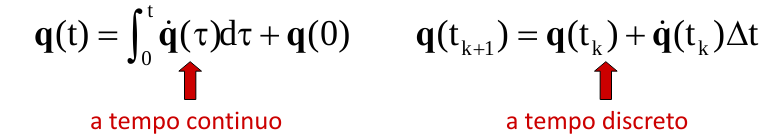
\includegraphics[width=0.7\linewidth]{images/diff_kine_11}
	\label{fig:diffkine11}
\end{figure}
e inserendo la forma di $\bm{q}$ ottenuta tramite lo Jacobiano (geometrico):
\begin{figure}[H]
	\centering
	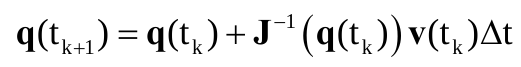
\includegraphics[width=0.4\linewidth]{images/diff_kine_12}
	\label{fig:diffkine12}
\end{figure}

Il problema con questa soluzione \textit{naïve} è che a causa di errori numerici divergeremo dalla soluzione voluta:
\begin{equation}\label{eq:inv_kine_diff_error}
\bm{e} = \bm{x}_d - \bm{x}
\end{equation}
Per risolvere il problema possiamo andare ad analizzare la dinamica d'errore:
\begin{equation*}
\bm{\dot{e}} = \bm{\dot{x}}_d - \bm{\dot{x}} = \bm{\dot{x}}_d - \bm{J}_A(\bm{q})\dot{\bm{q}}
\tag{$\star$}
\end{equation*}
e "chiudere il loop" per avere un feedback e correggere questo drift (e quindi far si che $\bm{e} \to 0$). Da qui, per semplicità supponendo che $\bm{J}_A$ sia invertibile, possiamo porre:
$$
\bm{\dot{q}}
\triangleq
\bm{J}_A^{-1}(\bm{q}) ( \dot{\bm{x}}_d + \bm{K}\bm{e})
$$
e, sostituendo in ($\star$), otteniamo la seguente dinamica d'errore:
\begin{gather*}
\bm{\dot{e}} = \bm{\dot{x}}_d - \bm{J}_A(\bm{q}) ( \bm{J}_A^{-1}(\bm{q}) ( \dot{\bm{x}}_d + \bm{K}\bm{e}) ) \\
\Downarrow \\
\bm{\dot{e}} = -\bm{K}\bm{e} \\
\Downarrow \\
\bm{\dot{e}} + \bm{K}\bm{e} = 0
\end{gather*}
dove se $\bm{K} > 0$ abbiamo stabilità asintotica dell'errore ($\implies \bm{x} \to \bm{x}_d$). Questa strategia può essere utilizzata per implementare il controllo cinematico, e funziona per basse velocità.

\begin{figure}[!hb]
	\centering
	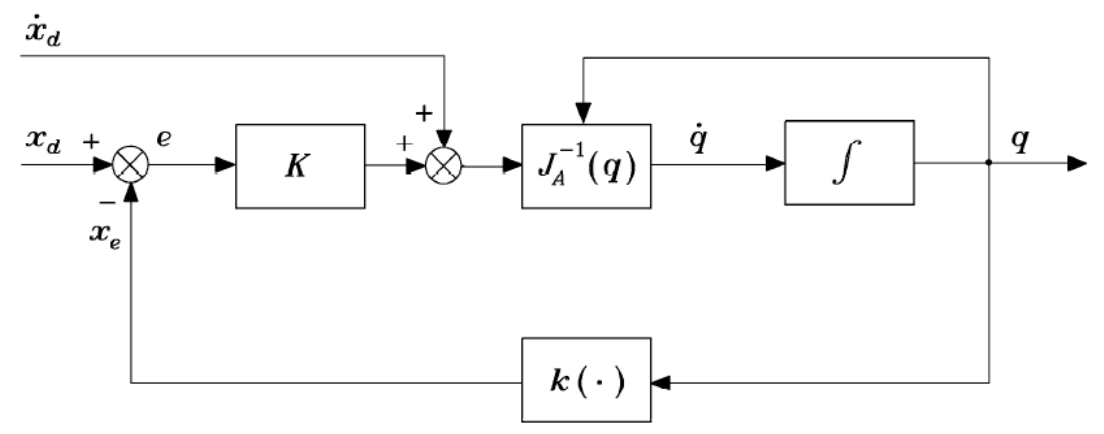
\includegraphics[width=0.7\linewidth]{images/diff_kine_13}
	\caption{Circuito di controllo con Jacobiano inverso e feedback}
	\label{fig:diffkine13}
\end{figure}




\subsection{Cinematica inversa tramite Jacobiano trasposto}
Nella soluzione tramite Jacobiano inverso stiamo in pratica usando una sorta di feedback linearization per trasformare la dinamica d'errore (non-lineare) in un'equazione lineare che possiamo facilmente controllare. Lo svantaggio principale di questa tecnica, è che richiede l'inversione di $\bm{J}(\bm{q})$, che (soprattutto nel di singolarità o ridondanza) è computazionalmente molto pesante.

Potremmo quindi pensare di progettare un "controllore" per l'errore direttamente nel caso non-lineare, ad esempio tramite il \textbf{metodo diretto di Lyapunov}. Scegliamo
$$
V(\bm{e})=\frac{1}{2}\bm{e}^{T}\bm{K}\bm{e} > 0 \quad \forall \bm{e} \neq \bm{0}
\qquad
,
\qquad
V(\bm{0}) = 0
$$
con $\bm{K} > 0$. Derivando e richiamando (\ref{eq:inv_kine_diff_error}), otteniamo:
$$
\dot{V}
=
\bm{e}^{T}\bm{K}\dot{\bm{x}}_{d} - \bm{e}^{T}\bm{K}\dot{\bm{x}}_{\bm{e}}
=
\bm{e}^{T}\bm{K}\dot{\bm{x}}_{d} - \bm{e}^{T}\bm{K} \underbrace{\bm{J}_A(\bm{q})\bm{\dot{q}}}_{\dot{\bm{x}}}
$$
e ponendo
$$
\dot{\bm{q}} \triangleq \bm{J}_{A}^{T}(\bm{q})\bm{K} \bm{e}
$$
otteniamo $\dot{V} < 0$ nel caso di riferimenti costanti ($\bm{x}_d = \text{const}$ i.e. $\bm{\dot{x}}_d = 0$).

\begin{figure}[!ht]
	\centering
	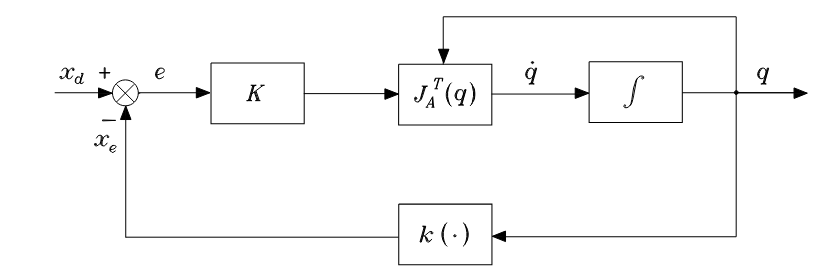
\includegraphics[width=0.7\linewidth]{images/diff_kine_14}
	\caption{Cinematica inversa con Jacobiano trasposto (riferimento costante)}
	\label{fig:diffkine14}
\end{figure}

Per il caso di $\bm{x}_d$ tempo-variante ($\bm{\dot{x}}_d \neq 0$), non riusciamo a garantire la convergenza dell'errore, che possiamo dire essere solo norm-bounded e inversamente proporzionale a $\bm{K}$. Per avere convergenza di tale errore dovremmo nuovamente scegliere $\dot{\bm{q}}$ dipendente dallo (pseudo-)inverso dello Jacobiano (quindi ritornando al caso di sez. \ref{section:invkineinvjac})